	\section{Exercise 2: Capacity estimation}

\begin{itshape}
\small
We now define the capacity of a Hopfield network of size N as the number of patterns $P_{N,max}$ that can be stored, such that the mean retrieval error averaged over all stored patterns (one retrieval attempt each) is at most 2$\%$. This yields the maximal load $\alpha_{N,max} = \frac{P_{N,max} }{N}$.

Set c=0.1. Calculate $\alpha_{N,max}$ for at least 10 network realizations and state the mean together with confidence intervals. Do this for N = 100, 250 and one other larger network size. Shortly interpret the resulting values and compare with results from literature.
\end{itshape}

\paragraph*{}

The results for $P_{N,max}$, $\alpha_{N,max}$ are shown in table \ref{tbl:exercise2_results} for N=100, 250 and 500.

\begin{table}[H] 
\centering 
\begin{table}[H] 
\centering 
\begin{tabular}{|l|l|l|l|l|l|l|} 
\hline 
N & tests & C-level & maximal load & lower bound & upper bound & $P_{N,max}$\\ 
 \hline \hline 
100 & 10 & 95.0 $ \% $& 0.1180 & 0.1163 & 0.1197 & 11.80 \\ 
250 & 10 & 95.0 $ \% $& 0.1252 & 0.1246 & 0.1258 & 31.30 \\ 
500 & 10 & 95.0 $ \% $& 0.1282 & 0.1279 & 0.1285 & 64.10 \\ 
\hline 
\end{tabular} 
\end{table} 

\label{tbl:exercise2_results}
\caption{The storage capacity $P_{N,max}$ and the maximal load $\alpha_{N,max}$ for 3 different pattern sizes N=(100,250,500).}
\end{table} 

\begin{figure}[htb] 
\centering
\begin{minipage}[c]{0.3\textwidth}
\centering 
\begin{tabular}{|l|l|}
\hline
$P_{error}$ & $\alpha_{N,max}$ \\ \hline \hline
0.001 & 0.105 \\
0.0036 & 0.138 \\
0.01 & 0.185 \\
0.05 & 0.37 \\
0.1 & 0.61 \\
\hline
\end{tabular}
\label{tbl:exercise2_lit_value}
\end{minipage}
\begin{minipage}[c]{0.69\textwidth}
\centering
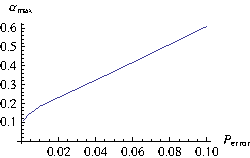
\includegraphics[width=0.69\textwidth]{dat/theovalues.pdf}
\end{minipage}
\caption{ The table on the left shows the literary values found in \citep{Hertz1991} and the figure on the right shows that $\alpha_{max}$ changes linearly in the region of $P_{error}=0.02$.}
\end{figure}



%p_max = 4.9477160735 * P_error + 0.1187211869 
% P_error = 0.02 : p_max = 0.22

Since the maximal load changes linearly around $P_{error}=0.02$ we can make a linear extrapolation and find that based on a linear expression this would mean $\alpha_{N,max} = 0.22$ for $P_{error}=0.02$. Our values are thus about half the literary values. It is to be expected that our values would be smaller than the literary values because the literary values are only upper bounds. This is because the calculation used for the literary values only considers the initial stability of the patterns. Of course as bits are flipped, these stabilities change, and one flipped bit can cause many other bits to flip and thereby create a sort of avalanche of bit flipping \citep[P. 19]{Hertz1991}. 